% LRC-BART presentation.
% Style reference: Yuan Ji, ENAR 2022 BaySize talk.
% Scientific source: MAP-BART revision/05-writing, September 2026.
\documentclass[11pt,aspectratio=169]{beamer}

\usepackage[english]{babel}
\usepackage[T1]{fontenc}
\usepackage{amsmath,amssymb,bm,mathtools}
\usepackage{booktabs,multirow}
\usepackage{graphicx}
\usepackage[round]{natbib}
\usepackage{xcolor}
\usepackage[absolute,overlay]{textpos}
\usepackage{tikz}
\usetikzlibrary{arrows.meta,positioning}

\newcommand{\Normal}{\mathrm{N}}
\newcommand{\E}{\mathbb{E}}
\newcommand{\Prb}{\mathbb{P}}
\newcommand{\bx}{\bm{x}}
\newcommand{\given}{\,\vert\,}
\newcommand{\target}{N_{\mathrm{target}}}
\newcommand{\Ber}{\mathrm{Bernoulli}}

\definecolor{UChicagoMaroon}{RGB}{128,0,0}
\definecolor{AccentBlue}{RGB}{0,75,135}
\definecolor{PFSRed}{HTML}{C1272D}
\definecolor{OSBlue}{HTML}{0000A7}
\definecolor{SoftGray}{RGB}{245,245,245}
\definecolor{MidGray}{RGB}{95,95,95}
\definecolor{BayesGreen}{RGB}{0,80,0}
\definecolor{BayesLight}{RGB}{236,244,236}
\definecolor{BayesGold}{RGB}{176,125,0}

\mode<presentation>{
  \usetheme{default}
  \usefonttheme{professionalfonts}
  \setbeamercolor{normal text}{fg=black,bg=white}
  \setbeamercolor{structure}{fg=UChicagoMaroon}
  \setbeamercolor{frametitle}{fg=UChicagoMaroon,bg=white}
  \setbeamercolor{title}{fg=black}
  \setbeamercolor{alerted text}{fg=UChicagoMaroon}
  \setbeamercolor{footline}{fg=black,bg=white}
  \setbeamerfont{frametitle}{size=\Large,series=\mdseries}
  \setbeamerfont{title}{size=\LARGE,series=\bfseries}
  \setbeamerfont{subtitle}{size=\normalsize}
  \setbeamerfont{footline}{size=\tiny}
  \setbeamersize{text margin left=0.65cm,text margin right=0.65cm}
  \setbeamertemplate{navigation symbols}{}
  \setbeamertemplate{itemize item}{\color{UChicagoMaroon}$\blacktriangleright$}
  \setbeamertemplate{itemize subitem}{\color{UChicagoMaroon}$\blacktriangleright$}
  \setbeamertemplate{enumerate item}{\color{UChicagoMaroon}\insertenumlabel.}
  \setbeamertemplate{frametitle}{
    \vspace{0.10cm}
    \hspace{-0.08cm}\insertframetitle\par
    \vspace{-0.18cm}
  }
  \addtobeamertemplate{frametitle}{}{%
    \begin{textblock*}{0.62cm}(15.12cm,0.10cm)
      
\includegraphics[width=0.58cm]{inserts/ucseal.pdf}
    \end{textblock*}}
  \setbeamertemplate{footline}{
    \ifnum\insertframenumber>1
      \leavevmode
      \vbox{%
        \hspace{0.35cm}\rule{15.3cm}{0.22pt}\par
        \vspace{0.05cm}
        \hbox to \paperwidth{%
          \hspace{0.4cm}\usebeamerfont{footline}\textbf{Yuan Ji}\quad
          University of Chicago\quad JSM 2026
          \hfill \insertshorttitle\hfill
          \insertframenumber\hspace{0.4cm}}%
        \vspace{0.10cm}}
    \fi}
}

\newcommand{\key}[1]{{\color{AccentBlue}\textbf{#1}}}
\newcommand{\sectionframe}[1]{%
  \begin{frame}[plain]
    \vspace*{0.46\paperheight}
    \hspace*{0.65cm}{\LARGE\bfseries #1}
  \end{frame}}

\title[LRC-BART]{Locally Robust Commensurate BART\\for Borrowing External Controls}
\subtitle{Local compatibility and borrowing calibration}
\author{Yuan Ji}
\institute{Department of Public Health Sciences\\University of Chicago}
\date{Joint Statistical Meetings 2026}

\begin{document}

\begin{frame}[plain]
  \begin{columns}[c,onlytextwidth]
    \column{0.82\textwidth}
      {\usebeamerfont{title}\inserttitle\par}
      \vspace{0.45em}
      {\color{UChicagoMaroon}\rule{0.88\textwidth}{0.5pt}\par}
      \vspace{0.55em}
      {\usebeamerfont{subtitle}\color{MidGray}\insertsubtitle\par}
      \vspace{1.2em}
      {\large \insertauthor\par}
      \vspace{0.25em}
      {\small \insertinstitute\par}
      \vspace{0.7em}
      {\small Collaborators: Yunxuan Zhang (UChicago), Gu Mi (Sanofi), Ji Lin (Sanofi)\par}
      \vspace{0.25em}
      {\small \insertdate\par}
    \column{0.18\textwidth}
      \centering
      
\includegraphics[width=1.45cm]{inserts/ucseal.pdf}
  \end{columns}
\end{frame}

\section{Motivation}
\sectionframe{Why borrow external controls?}

\begin{frame}{What external controls can contribute}
  \large
  \begin{itemize}\setlength\itemsep{1.0em}
    \item More observations for the control response surface
    \item Greater precision when the external and trial populations agree
    \item A smaller concurrent control arm in settings where borrowing is justified
  \end{itemize}

  \vspace{1.0em}
  \centering
  \key{The gain depends on transportability.}
\end{frame}

\begin{frame}{Compatibility can vary across patients}
  \large
  An external control may agree with the trial for one patient profile and differ for another.

  \vspace{1.0em}
  \begin{itemize}\setlength\itemsep{0.8em}
    \item Eligibility criteria and care pathways can differ by patient group.
    \item Measured and unmeasured confounding can create regional shifts.
  \end{itemize}

  \vspace{0.9em}
  \centering
  \key{One study-level borrowing parameter cannot distinguish those regions.}
\end{frame}

\begin{frame}{Established priors borrow at the study level}
  \small
  \renewcommand{\arraystretch}{1.35}
  \begin{tabular}{p{0.23\textwidth}p{0.68\textwidth}}
    \toprule
    \textbf{Prior} & \textbf{Borrowing mechanism} \\
    \midrule
    MAP prior &
    Exchangeable study parameters, with a robust component that reduces borrowing under conflict
    \citep{Neuenschwander2010MAP,schmidli2014robust} \\
    Commensurate prior &
    $\theta\mid\theta_0\sim\Normal(\theta_0,1/\tau)$, with a spike-and-slab prior on $\tau$
    \citep{Hobbs2011,Hobbs2012} \\
    Power prior &
    Historical likelihood raised to a discount parameter $a_0$
    \citep{IbrahimChen2000} \\
    \bottomrule
  \end{tabular}

  \vspace{0.9em}
  \centering
  \key{LRC-BART lets borrowing change with the covariates.}

  \vfill
  {\scriptsize With one historical study, these forms are closely related under suitable parameterizations \citep{RoverFriede2025}.}
\end{frame}

\section{Model}
\sectionframe{A local discrepancy model}

\begin{frame}{The trial-control mean is \(f(\bx)+g(\bx)\)}
  \large
  RCT controls have $D_i=1$ and external controls have $D_i=2$:
  \[
    y_i=f(\bx_i)+\mathbb{I}\{D_i=1\}\,g(\bx_i)+\varepsilon_i,
    \qquad \varepsilon_i\sim\Normal(0,\sigma^2_{D_i}).
  \]

  \vspace{0.7em}
  \begin{description}\setlength\itemsep{0.8em}
    \item[\key{\(f(\bx)\)}] External-control response mean, fitted to both control sources
    \item[\key{\(g(\bx)\)}] Local discrepancy, informed by the RCT controls
  \end{description}

  \vfill
  {\small The decomposition follows Bayesian causal forests, with source membership replacing treatment \citep{Hahn2020BCF}.}
\end{frame}

% Diagram: one illustrative discrepancy tree, not a fitted partition.
\begin{frame}{The discrepancy changes across patient profiles}
\centering
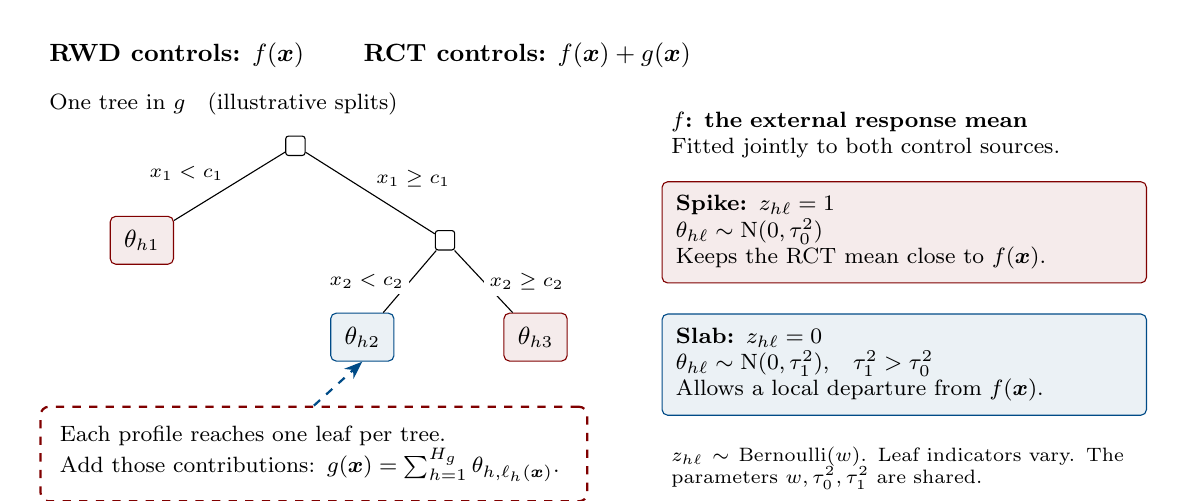
\begin{tikzpicture}[
  x=1cm,y=1cm,
  split/.style={draw,rounded corners=1pt,fill=white,minimum size=7pt,inner sep=1pt},
  spike/.style={draw=UChicagoMaroon,rounded corners=2pt,fill=UChicagoMaroon!8,inner sep=5pt,font=\small},
  slab/.style={draw=AccentBlue,rounded corners=2pt,fill=AccentBlue!8,inner sep=5pt,font=\small},
  edge label/.style={font=\scriptsize,fill=white,inner sep=2pt},
  note/.style={font=\footnotesize,align=left},
  callout/.style={draw=UChicagoMaroon,dashed,thick,rounded corners=3pt,fill=white,inner sep=7pt,align=left,font=\footnotesize}]
\path[use as bounding box] (0,0) rectangle (14.5,5.65);
\node[anchor=west,font=\small] at (0.15,5.3)
  {\textbf{RWD controls:} $f(\bx)$ \qquad \textbf{RCT controls:} $f(\bx)+g(\bx)$};
\node[anchor=west,note] at (0.15,4.68) {One tree in $g$ \; (illustrative splits)};
\node[split] (root) at (3.4,4.15) {};
\node[spike] (left) at (1.45,2.95) {$\theta_{h1}$};
\node[split] (right) at (5.3,2.95) {};
\node[slab] (middle) at (4.25,1.72) {$\theta_{h2}$};
\node[spike] (last) at (6.45,1.72) {$\theta_{h3}$};
\draw (root) -- (left) node[midway,edge label,above left] {$x_1<c_1$};
\draw (root) -- (right) node[midway,edge label,above right] {$x_1\ge c_1$};
\draw (right) -- (middle) node[midway,edge label,left] {$x_2<c_2$};
\draw (right) -- (last) node[midway,edge label,right] {$x_2\ge c_2$};
\node[callout,anchor=north west,text width=6.45cm] (sum) at (0.15,0.85)
  {Each profile reaches one leaf per tree.\\
   Add those contributions: $g(\bx)=\sum_{h=1}^{H_g}\theta_{h,\ell_h(\bx)}$.};
\draw[AccentBlue,dashed,thick,-{Stealth}] (sum.north) -- (middle.south);
\node[note,anchor=north west,text width=6.05cm] at (8.05,4.7)
  {\textbf{$f$: the external response mean}\\
   Fitted jointly to both control sources.};
\node[spike,anchor=north west,text width=5.8cm,align=left,font=\footnotesize] at (8.05,3.70)
  {\textbf{Spike: $z_{h\ell}=1$}\\
   $\theta_{h\ell}\sim\Normal(0,\tau_0^2)$\\
   Keeps the RCT mean close to $f(\bx)$.};
\node[slab,anchor=north west,text width=5.8cm,align=left,font=\footnotesize] at (8.05,2.02)
  {\textbf{Slab: $z_{h\ell}=0$}\\
   $\theta_{h\ell}\sim\Normal(0,\tau_1^2)$,\quad $\tau_1^2>\tau_0^2$\\
   Allows a local departure from $f(\bx)$.};
\node[note,anchor=north west,text width=6cm,font=\scriptsize] at (8.05,0.45)
  {$z_{h\ell}\sim\Ber(w)$. Leaf indicators vary. The parameters $w,\tau_0^2,\tau_1^2$ are shared.};
\end{tikzpicture}
\end{frame}


\begin{frame}{Each leaf can stay close or depart}
  \large
  A leaf contribution to $g=f_1-f$ follows
  \[
    \theta_{h\ell}\given w,\tau_0^2,\tau_1^2
    \stackrel{\mathrm{iid}}{\sim}
    w\,\Normal(0,\tau_0^2)+(1-w)\,\Normal(0,\tau_1^2),
    \qquad \tau_0^2<\tau_1^2.
  \]

  \vspace{0.7em}
  \begin{description}\setlength\itemsep{0.9em}
    \item[\key{Spike}] Small variance $\tau_0^2$ draws the trial-control mean toward $f(\bx)$.
    \item[\key{Slab}] Large variance $\tau_1^2$ permits a local departure from $f(\bx)$.
  \end{description}
\end{frame}

\begin{frame}{The indicator \(z_{h\ell}\) chooses the component}
  \large
  \[
    z_{h\ell}\mid w\sim\Ber(w),\qquad
    \theta_{h\ell}\mid z_{h\ell}
    \sim\Normal\!\left(0,\tau_{1-z_{h\ell}}^2\right).
  \]

  \vspace{0.8em}
  \begin{description}\setlength\itemsep{1.0em}
    \item[\key{\(z_{h\ell}=1\)}] Spike variance $\tau_0^2$: local commensurability
    \item[\key{\(z_{h\ell}=0\)}] Slab variance $\tau_1^2$: local conflict
  \end{description}

  \vfill
  {\small In the simulations, $f$ uses $H_f=50$ trees and $g$ uses $H_g=5$ shallow trees. The application uses $H_f=10$ and $H_g=5$.}
\end{frame}

\begin{frame}{The prior for \(f_1(\bx)\) remains centered at \(f(\bx)\)}
  \normalsize
  At a fixed profile, each discrepancy tree contributes one leaf. If $m$ of the $H_g$ reached leaves select the spike,
  \[
  \begin{split}
  f_1(\bx)\mid f,T_g,w,\tau_0^2,\tau_1^2
  \sim \sum_{m=0}^{H_g}
  &\binom{H_g}{m}w^m(1-w)^{H_g-m}\\[-0.2em]
  &\times\Normal\!\left(f(\bx),
      m\tau_0^2+(H_g-m)\tau_1^2\right).
  \end{split}
  \]

  \vspace{0.4em}
  \begin{itemize}\setlength\itemsep{0.45em}
    \item All components have mean $f(\bx)$.
    \item More slab leaves produce a wider prior for the latent trial-control mean.
    \item Observation variance remains separate.
  \end{itemize}
\end{frame}

\begin{frame}{Posterior computation follows standard BART moves}
  \large
  \begin{enumerate}\setlength\itemsep{0.75em}
    \item Update the trees for the shared response surface $f$.
    \item Update the shallow discrepancy trees for $g$.
    \item Draw each leaf indicator $z$, then its leaf mean $\theta$.
    \item Update the spike scale $\tau_0^2$ and mixture weight $w$.
  \end{enumerate}

  \vspace{0.6em}
  \begin{itemize}\setlength\itemsep{0.45em}
    \item The finite Gaussian mixture gives exact collapsed factors for tree moves.
    \item Log-normal AFT augmentation handles right-censored outcomes.
  \end{itemize}

  \vfill
  {\small Exact posterior invariance does not establish finite-chain mixing.}
\end{frame}

\section{Borrowing calibration}
\sectionframe{Calibrating the amount of borrowing}

\begin{frame}{Calibration targets the standardized control mean}
  \large
  For trial profiles $\bx_1,\ldots,\bx_N$,
  \[
    \mu=\frac{1}{N}\sum_{i=1}^N f_1(\bx_i).
  \]

  Let $V_\mu^f$ denote the RWD-only posterior variance of the standardized mean of $f$. The working prior ESS is
  \[
    \mathrm{ESS}_0(s_0^2)
    =\hat\sigma_1^2\,
      \E_{\tau_0^2}\!\left[
      \frac{1}{V_\mu^f+c_gH_g\tau_0^2}\right].
  \]

  \vfill
  {\small This variance-ratio summary is motivated by ELIR \citep{neuenschwander2020}, but it is not exact marginal ELIR for the BART scale mixture.}
\end{frame}

\begin{frame}{The fitted ceiling limits the ESS target}
  \large
  The largest working ESS is
  \[
    \frac{\hat\sigma_1^2}{V_\mu^f}.
  \]

  \vspace{0.7em}
  \begin{itemize}\setlength\itemsep{0.75em}
    \item The ceiling depends on the external-data fit at the trial profiles.
    \item The Pr-rule selects a scale for which working ESS is at or below the target in at least 95\% of blocks.
    \item A target at or above the whole-chain ceiling triggers the smallest-scale override.
  \end{itemize}

  \vfill
  {\small Equality to a scaled external sample size requires restrictive special cases.}
\end{frame}

\begin{frame}{Realized ESS uses the learned leaves}
  \normalsize
  For target-profile leaf proportions $a_{h\ell}$,
  \[
    V_g=\sum_{h,\ell}a_{h\ell}^2
    \left\{z_{h\ell}\tau_0^2+(1-z_{h\ell})\tau_1^2\right\}.
  \]
  The realized diagnostic averages
  \[
    \frac{\sigma_1^2}{V_\mu^f+V_g}
  \]
  over posterior draws.

  \vspace{0.6em}
  \begin{itemize}\setlength\itemsep{0.55em}
    \item Standardization can span several leaves in each tree.
    \item Regional ESS values use different standardized means and are not additive.
  \end{itemize}
\end{frame}

\begin{frame}{The borrowing map reports local compatibility}
  \large
  \[
    \mathcal B_c(\bx)
    =P\!\left\{|g(\bx)|<c\mid\text{data}\right\}.
  \]

  \vspace{0.7em}
  \begin{itemize}\setlength\itemsep{0.75em}
    \item $c$ is fixed in advance on the outcome scale.
    \item We report the map with the posterior mean and interval for $g(\bx)$.
    \item In the simulations, $c=0.5$, one third of the RCT residual SD for Gaussian outcomes.
  \end{itemize}

  \vfill
  {\small The map is a posterior probability. It is not the number of external patients used at a profile.}
\end{frame}

\begin{frame}{The theoretical results are conditional}
  \large
  \begin{description}\setlength\itemsep{0.8em}
    \item[\key{Influence}] The spike-and-slab leaf estimate has bounded local influence, and the spike effect vanishes under growing conflict.
    \item[\key{Detection}] With fixed partitions, fixed $f$, a representable discrepancy and growing local counts, the map separates compatible and incompatible regions.
    \item[\key{Calibration}] Under the untruncated scale law, working ESS decreases continuously from its ceiling to zero.
  \end{description}

  \vfill
  {\small These results do not establish full-posterior map consistency over learned partitions. Truncation gives a positive lower ESS limit.}
\end{frame}

\section{Simulation evidence}
\sectionframe{Simulation evidence}

\begin{frame}{Simulation settings}
  \large
  \begin{description}\setlength\itemsep{0.65em}
    \item[\key{Replicates}] $R=500$ paired trials
    \item[\key{Covariates}] $p=10$ with a nonlinear outcome surface
    \item[\key{External controls}] 300 patients
    \item[\key{Gaussian trial}] 200 treated and 100 controls, with $\sigma_1=1.5$ and $\sigma_2=1.8$
    \item[\key{Survival trial}] 225 treated and 75 controls, using log-normal AFT with about one quarter censored
    \item[\key{ESS targets}] 50, 75 and 100, plus 0.25, 0.5 and 0.9 of the fitted ceiling
  \end{description}
\end{frame}

\begin{frame}{Five compatibility scenarios}
  \normalsize
  \begin{description}\setlength\itemsep{0.58em}
    \item[\key{Sc1}] Source at random
    \item[\key{Sc2}] Source depends on measured covariates $(X_5,X_6)$
    \item[\key{Sc3}] Source and outcome depend on unmeasured $\bm U$, observed through proxies
    \item[\key{Sc4}] The external-control surface shifts outside $\mathcal R=\{X_5>2\}$
    \item[\key{Sc5}] The external-control surface shifts everywhere
  \end{description}

  \vspace{0.6em}
  \begin{itemize}\setlength\itemsep{0.4em}
    \item Gaussian Sc4 uses $\delta_2\in\{0.5,1,2\}$. Sc5 uses $\delta_2\in\{1,2\}$.
    \item Survival Sc4 uses $\delta_2\in\{0.5,1\}$. Sc5 uses $\delta_2=1$.
  \end{itemize}
\end{frame}

\begin{frame}{Gaussian outcomes}
  \small
  \centering
  \renewcommand{\arraystretch}{1.18}
  \setlength{\tabcolsep}{5.2pt}
  \begin{tabular}{lrr|rr}
    \toprule
    & \multicolumn{2}{c|}{LRC-BART (100)} & \multicolumn{2}{c}{BART-PP} \\
    Scenario & RMSE & Coverage & RMSE & Coverage \\
    \midrule
    Sc1: agreement & 0.17 & 0.94 & 0.21 & 0.94 \\
    Sc3: unmeasured conflict & 0.28 & 0.94 & 0.27 & 0.94 \\
    Sc4: regional, $\delta_2=1$ & 0.22 & 0.89 & 0.21 & 0.95 \\
    Sc4: regional, $\delta_2=2$ & 0.20 & 0.92 & 0.21 & 0.96 \\
    Sc5: global, $\delta_2=2$ & 0.20 & 0.92 & 0.21 & 0.95 \\
    \bottomrule
  \end{tabular}

  \vspace{0.75em}
  \begin{itemize}\setlength\itemsep{0.45em}
    \item Under agreement, LRC-BART lowers RMSE by about 16\% relative to BART-PP.
    \item Under global conflict, it suppresses borrowing and keeps bias near zero.
    \item A moderate regional shift remains the difficult case.
  \end{itemize}

  \vfill
  {\scriptsize BART-PP pools trial and external controls and includes a source indicator as a predictor.}
\end{frame}

\begin{frame}{Borrowing under a regional shift}
  \centering
  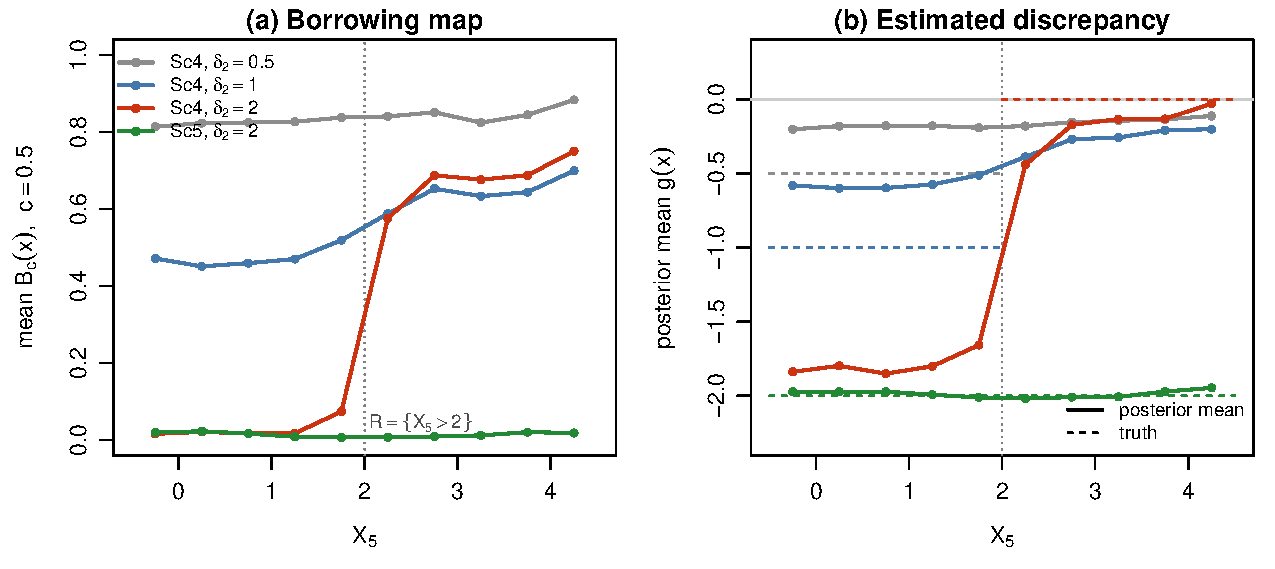
\includegraphics[width=0.86\textwidth]{inserts/lrc_fig_sc4_map.pdf}

  \vspace{0.25em}
  \small
  At $\delta_2=2$, mean compatibility is $0.02$ outside $\mathcal R$ and $0.70$ inside. The posterior mean discrepancy is $-1.8$ and $-0.15$, compared with truths $-2$ and $0$.

  \vfill
  {\scriptsize LRC-BART target 100, first 40 replicates. The transition spans about one unit of $X_5$ around the boundary.}
\end{frame}

\begin{frame}{Regional conflict remains the difficult case}
  \large
  \begin{columns}[T,onlytextwidth]
    \column{0.48\textwidth}
      \textbf{\color{UChicagoMaroon}Moderate shift: \(\delta_2=1\)}

      \vspace{0.35em}
      ATE bias is $-0.04$, coverage is $0.89$, and RMSE is $0.223$ versus $0.207$ for BART-PP.

    \column{0.48\textwidth}
      \textbf{\color{UChicagoMaroon}Strong shift: \(\delta_2=2\)}

      \vspace{0.35em}
      ATE bias is approximately zero. Compatible-region surface RMSE is $0.824$ versus $0.785$ for BART-PP.
  \end{columns}

  \vspace{1.0em}
  \begin{itemize}\setlength\itemsep{0.55em}
    \item Realized regional ESS is $9.5$ inside the compatible region and $0.44$ outside.
    \item The map is informative even when local surface estimation remains imperfect.
  \end{itemize}

  \vfill
  {\scriptsize Surface and regional ESS comparisons use $R=200$ paired replicates.}
\end{frame}

\begin{frame}{Survival outcomes}
  \small
  \centering
  RMST ratio at $t^\ast=3$, based on $R=500$ trials

  \vspace{0.3em}
  \renewcommand{\arraystretch}{1.14}
  \setlength{\tabcolsep}{7pt}
  \begin{tabular}{lrr}
    \toprule
    Scenario & LRC-BART RMSE & BART-PP RMSE \\
    \midrule
    Sc1: agreement & 0.097 & 0.106 \\
    Sc2: measured confounding & 0.100 & 0.097 \\
    Sc3: unmeasured confounding & 0.146 & 0.137 \\
    Sc4: regional shift & 0.108 & 0.113 \\
    Sc5: global shift & 0.112 & 0.110 \\
    \bottomrule
  \end{tabular}

  \vspace{0.7em}
  \begin{itemize}\setlength\itemsep{0.45em}
    \item Under agreement, power is $0.28$ for LRC-BART and $0.17$ for BART-PP.
    \item Coverage ranges from $0.90$ to $0.94$ for LRC-BART across these scenarios.
    \item Median-ratio estimation is less favorable under unmeasured confounding.
  \end{itemize}
\end{frame}

\begin{frame}{A single-arm study cannot learn the control discrepancy}
  \large
  Without an internal control arm, the trial contributes no data about $g(\bx)$.

  \vspace{0.9em}
  \begin{itemize}\setlength\itemsep{0.75em}
    \item Under no confounding, BART-CP and LRC-BART both have Gaussian RMSE $0.16$.
    \item Under measured confounding, every method is biased: ATE bias is $1.68$ for LM-CP, $0.41$ for BART-CP and $0.42$ for LRC-BART.
    \item The primary single-arm analysis fixes $w=1$ and interprets the result as borrowing from the external-control model.
  \end{itemize}

  \vfill
  {\small In Sc2, the fitted ceiling is 27 to 34, so an absolute target of 100 is capped.}
\end{frame}

\section{EloKRd application}
\sectionframe{EloKRd and the UCMM registry}

\begin{frame}{Trial and registry cohorts}
  \large
  \begin{columns}[T,onlytextwidth]
    \column{0.47\textwidth}
      \textbf{\color{UChicagoMaroon}EloKRd phase II trial}
      \begin{itemize}\setlength\itemsep{0.55em}
        \item 30 patients, all treated with EloKRd
        \item 13 PFS events and 10 deaths
        \item 50\% high-risk cytogenetics
        \item 30\% received ASCT
      \end{itemize}

    \column{0.47\textwidth}
      \textbf{\color{UChicagoMaroon}UCMM registry control}
      \begin{itemize}\setlength\itemsep{0.55em}
        \item 253 patients after cohort restrictions
        \item Standard induction regimens
        \item Five baseline covariates
        \item ASCT recorded after induction
      \end{itemize}
  \end{columns}

  \vfill
  \centering
  \key{Estimand: standardized five-year RMST ratio}
\end{frame}

\begin{frame}{Application analysis}
  \large
  \begin{itemize}\setlength\itemsep{0.72em}
    \item Analyze PFS and OS through the standardized five-year RMST ratio.
    \item Fit $H_f=10$ shared trees and $H_g=5$ shallow discrepancy trees.
    \item Compare working ESS targets of $15$ and $30$ with a target set at $90\%$ of the fitted ceiling.
    \item Report posterior intervals and $P(\text{RMST ratio}>1)$.
  \end{itemize}

  \vfill
  {\small ASCT is recorded after induction. The adjusted analysis is therefore a descriptive comparison conditional on recorded profiles, not a total causal treatment effect.}
\end{frame}

\begin{frame}{EloKRd: five-year RMST ratios}
  \small
  \centering
  \setlength{\tabcolsep}{6pt}
  \renewcommand{\arraystretch}{1.12}
  \begin{tabular}{lcc}
    \toprule
    Primary analysis & PFS & OS \\
    \midrule
    Kaplan--Meier, unadjusted & 1.01 (0.84, 1.22) & 0.90 (0.79, 1.03) \\
    Complete-pooling AFT & 0.87 (0.69, 1.06) & 0.80 (0.65, 0.94) \\
    Hierarchical AFT & 1.23 (0.74, 1.90) & 1.21 (0.77, 1.70) \\
    AFT-BART, no discrepancy & 0.97 (0.79, 1.16) & 0.90 (0.78, 1.02) \\
    \midrule
    \textbf{LRC-BART, \(\target=30\)} & \textbf{0.97 (0.77, 1.23)} & \textbf{0.90 (0.77, 1.04)} \\
    LRC-BART, $\target=15$ & 0.99 (0.75, 1.40) & 0.91 (0.76, 1.11) \\
    LRC-BART, $0.9\times$ ceiling & 0.97 (0.79, 1.15) & 0.90 (0.77, 1.04) \\
    \bottomrule
  \end{tabular}

  \vspace{0.8em}
  \raggedright
  At target 30, $P(\text{ratio}>1)$ is $0.37$ for PFS and $0.08$ for OS. Both nonparametric intervals include one.
\end{frame}

\begin{frame}{Local ESS at the trial profiles}
  \centering
  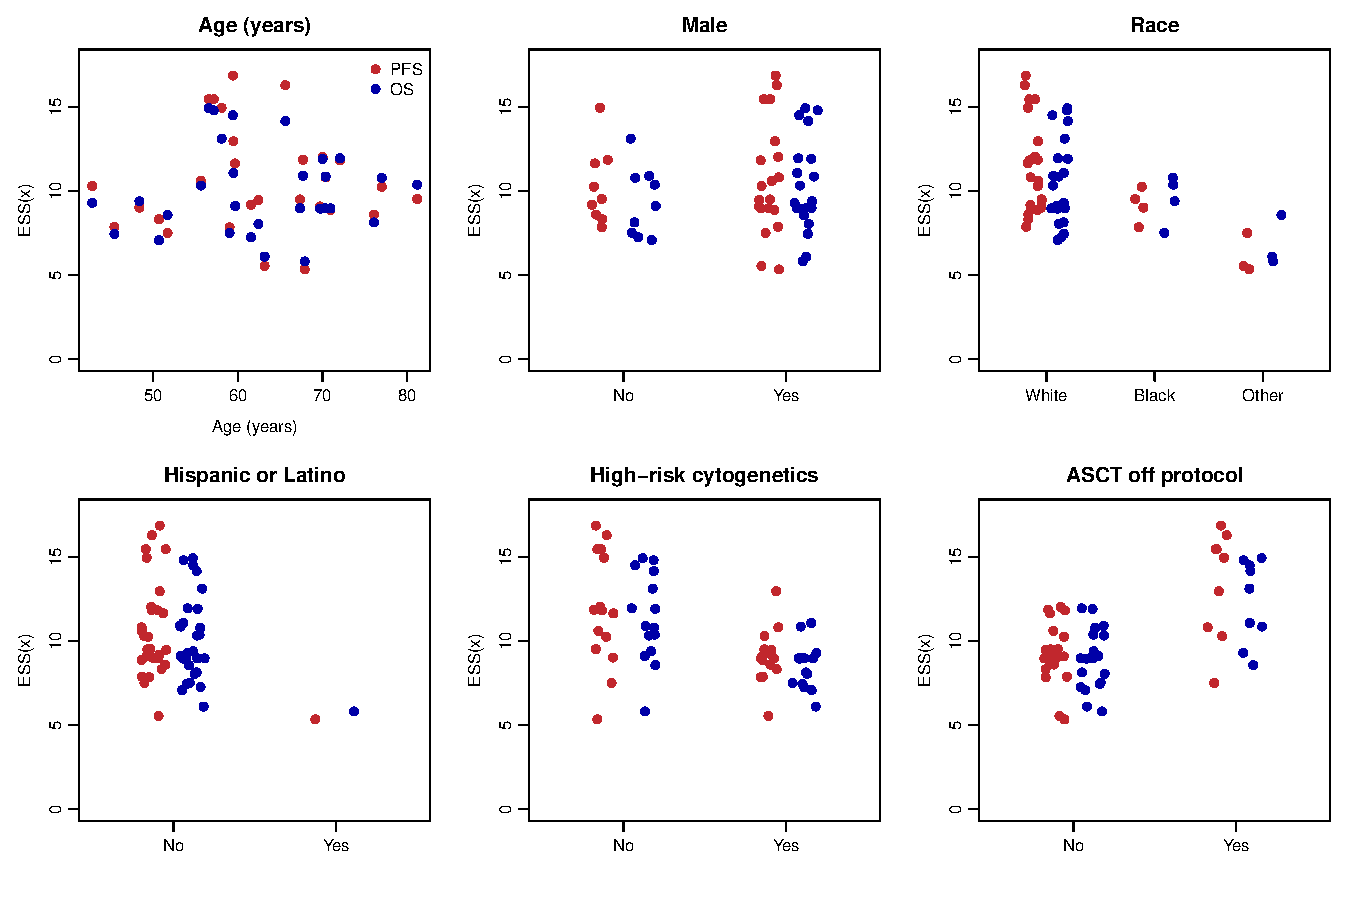
\includegraphics[height=0.55\textheight]{inserts/lrc_fig_ess_map.pdf}

  \vspace{0.15em}
  \normalsize
  {\color{PFSRed}$\boldsymbol{\bullet}$ PFS}\qquad
  {\color{OSBlue}$\boldsymbol{\bullet}$ OS}

  \vspace{0.3em}
  \raggedright\small
  Each dot is the local $\mathrm{ESS}(x)$ for one of the 30 EloKRd profiles. Higher values mean that more UCMM control information is transferred for that patient profile.

  \vspace{0.25em}
  {\scriptsize The same 30 profiles appear in every panel. Horizontal jitter for categorical covariates only separates overlapping dots. Values range from $5$ to $17$ for PFS and from $6$ to $15$ for OS; local values are not additive.}
\end{frame}

\section{Takeaways}
\begin{frame}{Main findings}
  \large
  \begin{enumerate}\setlength\itemsep{0.9em}
    \item A sparse discrepancy ensemble lets borrowing vary across patient profiles.
    \item The ESS calibration targets the standardized control mean and respects a fitted ceiling.
    \item Simulations show a precision gain under agreement and strong protection under global conflict. Moderate regional shifts remain the hard case.
  \end{enumerate}

  \vspace{0.9em}
  \centering
  \key{The map shows where the model regards the sources as compatible.}
\end{frame}

\begin{frame}{Limitations}
  \large
  \begin{itemize}\setlength\itemsep{0.78em}
    \item Map consistency is conditional on fixed partitions and a fixed shared surface.
    \item The ESS calibration is a working variance summary rather than exact marginal ELIR.
    \item A single-arm trial cannot identify the control discrepancy.
    \item Confirmatory use requires pre-specified operating-characteristic evaluation and a defined role for the borrowing map.
  \end{itemize}

  \vfill
  {\small Multiple external sources also require joint calibration. Additive ESS ceilings have not been established.}
\end{frame}

\begin{frame}[allowframebreaks]{References}
  \fontsize{7pt}{8pt}\selectfont
  \bibliographystyle{unsrtnat}
  \bibliography{ref_lrcbart}
\end{frame}

\appendix
\section{Technical backup}
\sectionframe{Technical backup}

\begin{frame}{Leaf hyperpriors and nested cases}
  \small
  \[
    w\sim\mathrm{Beta}(1,1),\qquad
    \tau_0^2\sim\text{scaled-Inv-}\chi^2(\nu_0,s_0^2)
    \ \text{truncated to }(0,\tau_1^2),
  \]
  with $\tau_1^2$ fixed by the range rule.

  \vspace{0.7em}
  \begin{description}\setlength\itemsep{0.6em}
    \item[\key{\(w=1\)}] Commensurate BART (C-BART), with one learned spike scale
    \item[\key{\(w=1,\tau_0^2\to0\)}] Complete pooling BART (BART-CP)
    \item[\key{\(w=0\)}] A free source offset, analogous to BART with a source indicator (BART-PP)
  \end{description}

  \vfill
  {\scriptsize Appendix G.6 compares constrained joint prior modes over integer slab counts. It does not establish posterior indicator probabilities, which also depend on the likelihood and partitions.}
\end{frame}

\begin{frame}{Why use separate ensembles?}
  \large
  \begin{itemize}\setlength\itemsep{0.75em}
    \item The shared surface $f$ and discrepancy $g$ can use different partition and shrinkage priors.
    \item The simulations use $H_f=50$ trees and $H_g=5$ shallow trees, with split prior $(0.5,3)$ for $g$.
    \item At fixed leaf variances and partitions, fewer discrepancy trees reduce the all-spike variance at a profile.
    \item The slab range rule also depends on $H_g$.
  \end{itemize}

  \vfill
  {\small The simulation results assess this specification. They do not show that a shared-leaf model cannot detect regional discrepancies.}
\end{frame}

\begin{frame}{Calibration conventions and borrowing summaries}
  \small
  \begin{itemize}\setlength\itemsep{0.55em}
    \item The constant $c_g$ averages squared leaf proportions before inversion. The calibration scale law is untruncated.
    \item The working ESS and ceiling use the standardized control mean. The pointwise ESS uses a profile-specific posterior variance.
    \item The realized regional ESS uses posterior indicators and leaf proportions for its own standardized regional mean.
    \item $B(x)$, the probability that all reached leaves select the spike, remains a diagnostic. Its prior scale is $w^{H_g}$.
    \item A fixed positive spike scale need not identify compatibility through $B(x)$ as local RCT counts grow.
  \end{itemize}

  \vfill
  {\small Compatibility probability, prior ESS and realized regional ESS answer different questions. None is an observed count of external patients used.}
\end{frame}

\begin{frame}{Comparator labels}
  \normalsize
  \begin{description}\setlength\itemsep{0.55em}
    \item[\key{LM-PP}] Linear regression on pooled controls, with source indicator
    \item[\key{BART-NP}] Standard BART fitted to the RCT controls only
    \item[\key{BART-CP}] Standard BART fitted to pooled controls, without a source indicator
    \item[\key{BART-PP}] Standard BART fitted to pooled controls, with a source indicator
    \item[\key{C-BART}] LRC-BART with $w=1$, using one commensurate discrepancy scale
  \end{description}

  \vfill
  {\small The study also includes linear/AFT analogues, PSCL, MAP and hierarchical models.}
\end{frame}

\begin{frame}{Borrowing diagnostics in the Gaussian study}
  \small
  \begin{itemize}\setlength\itemsep{0.52em}
    \item Under Sc1, LRC-BART RMSE is $0.172$ versus $0.205$ for BART-PP. Prior ESS is $82$, the ceiling is $127$, and realized ESS is $53$.
    \item Under Sc3, realized ESS falls to $1.6$. Bias exceeds BART-PP by $0.012$ with paired SE $0.001$.
    \item Under Sc5 at $\delta_2=2$, the map averages $0.01$ and realized ESS is $0.2$.
    \item Under Sc2, the ceiling falls from $127$ to $23$, so all absolute targets are capped.
    \item Under Sc4 at $\delta_2=2$, surface RMSE away from the boundary is $0.747$ versus $0.723$, a difference of $0.024$ with SE $0.005$ over $R=200$ replicates.
  \end{itemize}
\end{frame}

\begin{frame}{Additional borrowing-map results}
  \large
  \begin{itemize}\setlength\itemsep{0.75em}
    \item At $\delta_2=1$, the mean map is $0.62$ inside $\mathcal R$ and $0.52$ outside. The posterior mean discrepancy is $-0.25$ and $-0.60$.
    \item At $\delta_2=0.5$, the map is nearly flat at $0.84$, below the stated resolution.
    \item Under the global shift Sc5 at $\delta_2=2$, the map is $0.01$ throughout the covariate space.
  \end{itemize}

  \vfill
  {\small A secondary Sc4 shift on the null covariate $X_7$ gives similar map and ATE results.}
\end{frame}

\begin{frame}{Exact leaf marginals for tree moves}
  \footnotesize
  Conditionally on $(\tau_0^2,\tau_1^2,w)$,
  \[
    M_f=(1+\lambda_f^2A)^{-1/2}
    \exp\left\{\frac{\lambda_f^2B^2}{2(1+\lambda_f^2A)}\right\},
  \]
  \[
    M_g=
    \frac{w\,\phi(\bar y_1;0,\tau_0^2+v_1)
    +(1-w)\,\phi(\bar y_1;0,\tau_1^2+v_1)}
    {\phi(\bar y_1;0,v_1)}.
  \]
  Here $A$ and $B$ are precision-weighted counts and sums from both sources in an $f$ leaf. The terms $\bar y_1$ and $v_1=\sigma_1^2/n_1$ are the RCT residual mean and variance in a $g$ leaf.

  \vspace{0.5em}
  Grow, prune and change moves use these collapsed ratios. One sweep costs a standard BART fit on $n_1+n_2$ observations plus a five-tree ensemble on $n_1$.
\end{frame}

\begin{frame}{Conditional bounds and consistency statements}
  \footnotesize
  Write $v=\sigma_1^2/n$ for an RCT residual-mean variance. The results condition on $f$, other discrepancy trees, partitions, scales and $0<w<1$.

  Let $a=\log\{(1-w)/w\}+\tfrac12\log\{(\tau_0^2+v)/(\tau_1^2+v)\}$ and $C=e^{-a}$.

  \vspace{0.4em}
  \begin{description}\setlength\itemsep{0.55em}
    \item[\key{Influence}] Relative to the slab estimate,
      $\sup_{\bar y}|I(\bar y)|\le
      \sqrt{2v\max\{\log C,\tfrac12\}}$.
      The shift vanishes at a Gaussian rate under growing conflict.
    \item[\key{Map}] With fixed partitions, fixed $f$, a representable discrepancy and growing local counts,
      $\mathcal B_c(x)\to\mathbb I\{|d|<c\}$ for $|d|\ne c$.
    \item[\key{ESS}] Under the untruncated law, $\mathrm{ESS}_0$ is continuous, convex and strictly decreasing from its ceiling to zero. Truncation gives a positive lower limit.
  \end{description}

  \vfill
  {\scriptsize A fixed positive spike scale need not identify compatibility through the all-spike indicator. Grid-selection consistency requires the stated moment and separation conditions.}
\end{frame}

\begin{frame}{Gaussian outcomes: full comparison}
  \centering
  \fontsize{6.4pt}{7.1pt}\selectfont
  \setlength{\tabcolsep}{2.7pt}
  \renewcommand{\arraystretch}{0.94}
  \resizebox{\textwidth}{!}{%
  \begin{tabular}{lrrr|rrr|rrr|rrr|rrr}
    \toprule
    & \multicolumn{3}{c|}{Sc1} & \multicolumn{3}{c|}{Sc3, $\rho=0$}
    & \multicolumn{3}{c|}{Sc4, $\delta_2=1$}
    & \multicolumn{3}{c|}{Sc4, $\delta_2=2$}
    & \multicolumn{3}{c}{Sc5, $\delta_2=2$} \\
    Method & Bias & RMSE & Cov & Bias & RMSE & Cov & Bias & RMSE & Cov
    & Bias & RMSE & Cov & Bias & RMSE & Cov \\
    \midrule
    LM-PP   & $-$0.00 & 0.34 & 0.94 & 0.04 & 0.35 & 0.95 & $-$0.01 & 0.34 & 0.95 & $-$0.02 & 0.34 & 0.95 & $-$0.04 & 0.34 & 0.94 \\
    BART-NP & 0.00 & 0.22 & 0.91 & $-$0.00 & 0.29 & 0.94 & 0.00 & 0.22 & 0.91 & 0.00 & 0.22 & 0.91 & 0.00 & 0.22 & 0.91 \\
    BART-CP & 0.01 & 0.14 & 0.96 & 0.98 & 1.00 & 0.00 & $-$0.34 & 0.37 & 0.35 & $-$0.68 & 0.70 & 0.00 & $-$1.39 & 1.40 & 0.00 \\
    BART-PP & 0.01 & 0.21 & 0.94 & 0.03 & 0.27 & 0.94 & $-$0.00 & 0.21 & 0.95 & $-$0.01 & 0.21 & 0.96 & $-$0.01 & 0.21 & 0.95 \\
    C-BART  & 0.01 & 0.15 & 0.95 & 0.23 & 0.38 & 0.87 & $-$0.21 & 0.27 & 0.73 & $-$0.23 & 0.39 & 0.66 & $-$0.32 & 0.65 & 0.76 \\
    \textbf{LRC-BART (100)} & \textbf{0.01} & \textbf{0.17} & \textbf{0.94}
      & \textbf{0.04} & \textbf{0.28} & \textbf{0.94}
      & $\bm{-0.04}$ & \textbf{0.22} & \textbf{0.89}
      & \textbf{0.00} & \textbf{0.20} & \textbf{0.92}
      & $\bm{-0.00}$ & \textbf{0.20} & \textbf{0.92} \\
    \bottomrule
  \end{tabular}}

  \vspace{0.45em}
  \raggedright
  {\scriptsize CAHB comparisons use the first $R=200$ paired Gaussian replicates and assess transfer of kernel-local estimation. They do not establish a general method ranking \citep{Jin2023CAHB}.}
\end{frame}

\begin{frame}{Survival outcomes: full RMST results}
  \centering
  \small
  RMST ratio at $t^\ast=3$, based on $R=500$ trials

  \vspace{0.25em}
  \setlength{\tabcolsep}{5.5pt}
  \renewcommand{\arraystretch}{1.02}
  \begin{tabular}{lrrr|rrr}
    \toprule
    & \multicolumn{3}{c|}{LRC-BART (100)} & \multicolumn{3}{c}{BART-PP} \\
    Scenario & Bias & RMSE & Cov & Bias & RMSE & Cov \\
    \midrule
    Sc1: agreement & 0.003 & 0.097 & 0.94 & $-$0.023 & 0.106 & 0.94 \\
    Sc2: measured confounding & 0.018 & 0.100 & 0.93 & $-$0.002 & 0.097 & 0.95 \\
    Sc3: unmeasured confounding & 0.031 & 0.146 & 0.94 & $-$0.005 & 0.137 & 0.92 \\
    Sc4: regional shift & $-$0.037 & 0.108 & 0.90 & $-$0.059 & 0.113 & 0.91 \\
    Sc5: global shift & 0.001 & 0.112 & 0.93 & $-$0.041 & 0.110 & 0.93 \\
    \bottomrule
  \end{tabular}

  \vspace{0.65em}
  {\small Sc3 uses $\rho=0$. Sc4 and Sc5 use $\delta_2=1$. Full results appear in the paper and Web Table S2.}
\end{frame}

\begin{frame}{Single-arm sensitivity details}
  \small
  The trial contributes treated subjects only ($n_T=200$ Gaussian and $30$ or $200$ survival), and the 300 external controls are the sole control source.

  \vspace{0.5em}
  \begin{itemize}\setlength\itemsep{0.5em}
    \item Under no confounding, the survival RMST ratio at $n_T=30$ has RMSE $0.16$ to $0.19$ and coverage $0.92$ to $0.97$.
    \item The fractional ESS target widens intervals. Coverage ranges from $0.82$ to $0.99$.
    \item With $w<1$, slab variance adds uncertainty: SD $1.4$ for the ATE and $10$ to $34$ for the median ratio.
    \item A zero-mean discrepancy preserves linear log-time means, but survival-ratio means can change.
    \item Hierarchical regressions give ATE SD $8$ under the stated hyperprior.
  \end{itemize}
\end{frame}

\end{document}
